\documentclass[../basic_graph_theory.tex]{subfiles}

\begin{document}
\chapter{Planarity}
\setcounter{chapter}{6} %Set chapter counter
\setcounter{section}{6}
\setcounter{equation}{6}
\setcounter{figure}{6}

A graph $G$ is said to be planar if it can be drawn in the plane in such a way that pairs of edges intersect only at vertices, if at all. If $G$ has no such representation, $G$ is called nonplanar. A drawing of a planar graph $G$ in the plane in which edges intersect only at vertices is called a planar representation (or a planar embedding) of $G$.\\

If three or more edges bound a portion of a graph then we call it a region. In figure \ref{fig:regions}, $R_1, R_2, \dots, R_7$ are regions in the graph. An edge $e$ bounds a region $R$, if it comes in contact with $R$. We denote the bound degree of $R$ by $b(R)$ and define it as the number of edges that bound region $R$.

\begin{figure}[hbt!]
    \label{fig:regions}
    \centering
    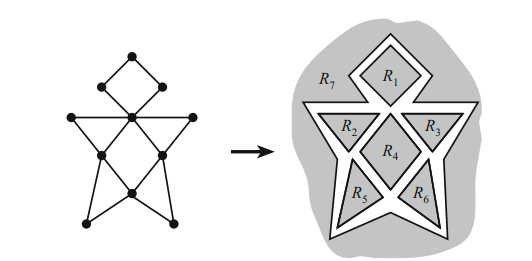
\includegraphics[height=4cm,width=9.5cm]{images/region.png}
    \caption{Representation of regions in a graph}
\end{figure}

Now, we are ready to state the famous Euler's formula.
\begin{thm}[Euler's formula]
    For a connected planar graph $G$ with $n$ vertices, $q$ edges, and $r$ regions, then $n-q+r=2$.
\end{thm}
\begin{proof}
    We induct on $q$, the number of edges. If $q = 0$, then $G$ must be $K_1$, a graph with $1$ vertex and $1$ region. The result holds in this case. Assume that the result is true for all connected planar graphs with fewer than $q$ edges, and assume that $G$ has $q$ edges.\\
    \em{Case 1.} Suppose $G$ is a tree. We know from our work with trees that $q = n-1$, and $r = 1$, since a planar representation of a tree has only one region. Thus, $n - q + r = n - (n - 1) + 1 = 2$, and the result holds.\\
    \em{Case 2.} Suppose $G$ is not a tree. Let $C$ be a cycle in $G$, let e be an edge of $C$, and consider the graph $G - e$. Compared to $G$, this graph has the same number of vertices, one edge fewer, and one region fewer, since removing e coalesces two regions in $G$ into one in $G - e$. Thus the induction hypothesis applies, and in $G - e$, $n - (q - 1) + (r - 1) = 2$, implying that $n - q + r = 2$.\\
    The result holds in both cases, and the induction is complete.
\end{proof}

Euler's formula helps us a lot in identifying non-planar graphs. We urge you to check using Euler's formula that $K_{3,3}$ and $K_5$ are non-planar. A more general general version of the Euler's formula has been stated below.

\begin{thm}
    For a planar graph $G$ with $n$ vertices, $q$ edges, and $r$ regions, then $n-q+r=1+\beta_{0}(G)$.
\end{thm}

\begin{thm}
    If $G$ is a planar graph with $n \ge 3$ vertices and $q$ edges, then $q \le 3n - 6$. Furthermore, if equality holds, then every region is bounded by three edges.
\end{thm}
\begin{proof}
    Let, us consider $C=\sum_{R}b(R)$.\\
    Since every edge of $G$ is shared by at most $2$ regions so, $C \le 2q$. Further as each region is bounded by atleast $3$ edges, so $C \ge 3r$. Thus,\\
    \begin{align*}
        &3r \le 2q\\
        \Longrightarrow &3(2+q-n) \le 2q\\
        \Longrightarrow &6+3q-3n \le 2q\\
        \Longrightarrow &q \le 3n-6\\
    \end{align*}
    If equality holds, then $3r = 2q$, and it must be that every region is bounded by three edges.
\end{proof}

\begin{thm}
    If $G$ is a planar graph, then $\delta(G) \le 5$.
\end{thm}
\begin{proof}
    Suppose $G$ has $n$ vertices and $q$ edges. If $n \le 6$, then the result is immediate, so we will suppose that $n > 6$. If we let $D$ be the sum of the degrees of the vertices of $G$, then we have:\\
    \begin{equation*}
        D = 2q \le 2(3n - 6) = 6n - 12
    \end{equation*}
    If each vertex had degree $6$ or more, then we would have $D \ge 6n$, which is impossible. Thus there must be some vertex with degree less than or equal to $5$.
\end{proof}

Now, we define what we mean by a subdivision as the concluding portion of this chapter will cover two theorems that are very important and will go a long way in helping us outright identify many graphs as non-planar.\\

\begin{defn}
    A subdivision of an edge $G$ is a substitution of a path for $e$.
\end{defn}
\begin{defn}
    We say that, $H$ is a subdivision of $G$ if $H$ can be obtained from $G$ by a finite sequence of subdivisions.
\end{defn}

Now that the idea of subdivisions has been introduced we can finally move on to the last two theorems for this chapter.
\begin{thm}
    A graph $G$ is planar iff every subdivision of $G$ is planar.
\end{thm}
The proof for this is very intuitive as so is left as an exercise for the reader.\\
Lastly, we end this chapter by stating and proving Kuratowski's theorem.\\
\begin{thm}
    A graph $G$ is planar iff it contains no subdivision of $K_{3,3}$ or $K_{5}$.
\end{thm}
We state this theorem without proof as the proof is not very easy. However, you acn check out the proof of Kuratowski's theorem online.

\end{document}